\section{Realised transport: what abstract loss does and does not mean}\label{sec:realised}
\Cref{cor:threestage} says that the abstract complex of the three-stage orbit loses every positive-dimensional cell. This section shows that the realised union behaves differently: edges are always retained, some squares are not.

\subsection{Lost edges are geometrically retained}
\begin{theorem}\label{thm:E28}
Let $\Lambda\subseteq\Z^k$ be any lattice and $Q$ a box with all $q_i\ge1$. Every cell of dimension $\le1$ of $\Kabs(\Lambda,Q)$ lies in $U(\Z^k,Q)$. In particular, for the even-sum lattice $E_k$ every edge segment $[u,u+g]$, $g\in\Gr(E_k)$, of $\Kabs(E_k,Q)$ lies in $U(\Z^k,Q)$, although (\cref{cor:threestage}) none of these edges is an edge of $\Kabs(\Z^k,Q)$.
\end{theorem}
\prov{CW-0463}{E2-8}{PROVED}{FULL}
\begin{proof}
$\Z^k$ is a rectangular target with all $o_i=1$ and $F(\Lambda,Q)\subseteq F(\Z^k,Q)$. By \cref{thm:corner}(d) no cell of dimension $\le1$ meets $O=[0,1)^k$, and by \cref{thm:corner}(a)--(b) a subset of $B=Q$ that misses $O$ lies in $U(\Z^k,Q)$. \qedhere
\end{proof}
The release states and proves this for $E_k$ by a direct coordinate argument; the form above is the corner-cube form of the same fact. For the specimen $k=3$, all $45$ lost edges were also tested at five interior points each by independent code (a check of the theorem, not an additional proof).
\begin{figure}[tbp]\centering
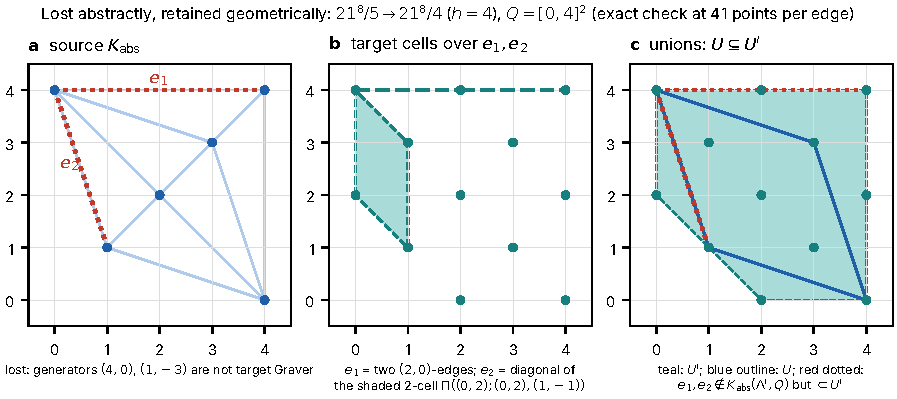
\includegraphics[width=0.98\textwidth]{fig07_lost_edges_retained}
\caption{Abstract loss versus realised containment (\cref{thm:E28} and \cref{thm:laws}(L3); planar specimen $21^{8}/5\to21^{8}/4$, $h=4$, $Q=[0,4]^2$; \emph{exact computation}, each edge checked exactly at $41$ points). (a)~Two edges $e_1$ (from $(0,4)$ to $(4,4)$, generator $(4,0)$) and $e_2$ (from $(0,4)$ to $(1,1)$, generator $(1,-3)$) of $\Kabs(\Lambda,Q)$, $\Lambda=\{a\equiv b\ (4)\}$; neither generator is Graver for $\Lambda'=\{a\equiv b\ (2)\}$, so both edges are lost in $\Kabs(\Lambda',Q)$. (b)~In the target complex $e_1$ is the union of two $(2,0)$-edges and $e_2$ is a diagonal of the shaded $2$-cell $\Pil((0,2);(0,2),(1,-1))$. (c)~The unions: $U(\Lambda',Q)$ (teal) contains $U(\Lambda,Q)$ (blue outline), and the lost edges (red, dotted) lie inside it. Distinct objects: lost in $\Kabs(\Lambda',Q)$, contained in $U(\Lambda',Q)$.}\label{fig:lost}
\end{figure}

\subsection{Cells that leave the union}
\begin{proposition}\label{prop:E29}\sloppy
Let $k=3$, $Q=[0,2]^3$. The parallelogram $c_*=\Pil((0,0,2);(0,1,-1),(1,0,-1))$ is a $2$-cell of $\Kabs(E_3,Q)$ (its corners $(0,0,2),(0,1,1),(1,0,1),(1,1,0)$ lie in $F(E_3,Q)$ and its generators are Graver). It contains $(\tfrac23,\tfrac23,\tfrac23)=(0,0,2)+\tfrac23(0,1,-1)+\tfrac23(1,0,-1)\in[0,1)^3$. Hence $U(E_3,Q)\not\subseteq U(\Z^3,Q)$ although $F(E_3,Q)\subseteq F(\Z^3,Q)$. Conversely $(1,0,0)\in U(\Z^3,Q)\setminus U(E_3,Q)$.
\end{proposition}
\prov{CW-0464}{E2-10}{FINITE-EXACT}{FINITE}
\begin{proof}
The first part is \cref{thm:evensum} for $\tilde Q=(2,2,2)$ and \cref{cor:E27}. For the converse, every nonzero point of $E_3$ has coordinate sum $\ge2$, hence so has every point of $U(E_3,Q)\subseteq\conv F(E_3,Q)$, while $(1,0,0)$ is a point of $F(\Z^3,Q)$. \qedhere
\end{proof}
(The proposition is carried by the source record E2-9, whose row is the same \texttt{CW-0464} area; the classification of \emph{which} source cells leave $U'$ --- exactly six, three squares and three cubes, all containing the three points $(0,1,1),(1,0,1),(1,1,0)$ --- is a finite exact computation of the release and is cited, not re-derived.)

\subsection{Finite findings on topology and specimens}
\begin{proposition}[FINITE-EXACT; scope: the $k=3$ specimen and two planar specimens]\label{prop:topology}
(a) For the specimen of \cref{prop:specimen} the Betti numbers of the abstract complexes are $(1,6,6,0)\to(1,0,0,0)$ while the fibre grows; the realised union of the source has Betti numbers $(1,0,18,0)$ (nerve computation of the release; cited). (b) For the planar specimen $21^8/5\to21^8/4$ ($h=4$) all $8$ abstractly lost edges and the lost square lie in $U'$, with $U\subsetneq U'$, realised Betti $(1,2,0)\to(1,0,0)$ while the abstract Betti numbers are $(1,5,0)\to(1,2,6)$; neither complex is embedded. (c) For the planar specimen $55^{12}/27\to55^{12}/18$ all $5$ source edges persist, $U$ is embedded with Betti $(1,0,0)$, but $U'$ is non-embedded with realised Betti $(1,2,0)$ (abstract $(1,8,0)$): enlargement can create holes.
\end{proposition}
\prov{CW-0474}{P2-G}{FINITE-EXACT}{FINITE}
Statement (a) first half was recomputed here; the other items are reported by the release and are not re-derived. The planar hole creation and destruction in (b),(c) are explained by frozen planar theory (the source lattices sit at the exceptional hollow box $(d,d)$ or below the stabilisation threshold; ER-19), so they are an observation about transport, not new single-fibre topology.

\subsection{Verdict on the plausible laws}
\begin{theorem}[laws refuted by exact witnesses]\label{thm:laws}
None of the following is true in general. (L1) $D(x)\subseteq D(x')$ implies persistence of Graver edges. (L2) $F\subseteq F'$ implies $U\subseteq U'$. (L3) Abstract loss of a cell implies that the cell leaves the target union. (L4) Topology of the abstract complex or of the union is monotone under inclusion of occurrence sets. (L5) A change of denominator changes the relation lattice.
\end{theorem}
\prov{CW-0465}{E2-11}{COUNTEREXAMPLE}{EXAMPLE}
\begin{proof}
(L1): \cref{cor:threestage}. (L2): \cref{prop:E29}. (L3): \cref{thm:E28}. (L4): \cref{prop:specimen} and \cref{prop:topology}: $b_1(\Kabs)$ falls from $6$ to $0$ and $b_2(U)$ from $18$ to $0$ while $F$ grows from $13$ to $26$ points (finite-exact specimen). (L5): for the primes $5,17,29$ the lattices for $b=3$ and $b=12$ coincide (\cref{cor:denominators}); the release's family of $405$ transitions of the three-stage type records $276$ EQUAL steps with denominator changes of this kind (finite-exact, cited). \qedhere
\end{proof}
\prov{CW-0475}{E2-P2-V}{PROVED}{EXAMPLE}
The release records six preregistered propositions P2-F1--P2-F6, each refuted by an exact witness; among them P2-F4 (abstract edge loss with full geometric containment, $199$ corpus rows) is the planar form of (L3) and P2-F5 (the planar pattern extends to $k=3$) is refuted by the witness of \cref{prop:E29}. The other verdicts are cited from the release and are not used below.
